\section{Introdução}
\begin{frame}
\frametitle{Grafo Simples}
\begin{columns}[T]
    \begin{column}{.75\textwidth}
       \resizebox{\textwidth}{!}{%
        \centering
        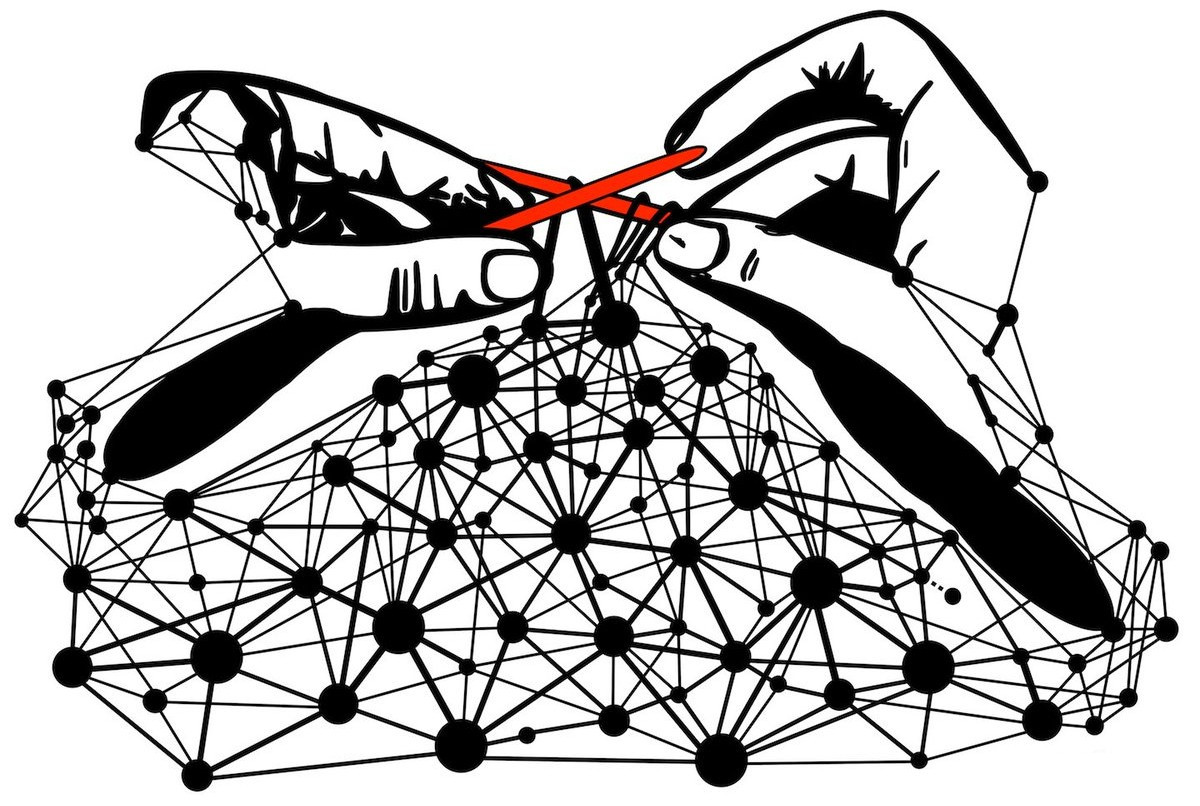
\includegraphics[scale=.5]{img/grafo-tranc.jpg}
    }
    \end{column}
    \begin{column}{.25\textwidth}
       \begin{itemize}
            \item{V(G): conjunto finito e não vazio de vértices}
            \item{E(G): pares não ordenados de elementos de V(G)}
            \item{Sem laços e multiarestas}
        \end{itemize}
    \end{column}
  \end{columns}
\end{frame}

\begin{frame}
\frametitle{Grafo}
\frametitle{Relações Sociais}
\centering
\resizebox{.7\textwidth}{!}{%
    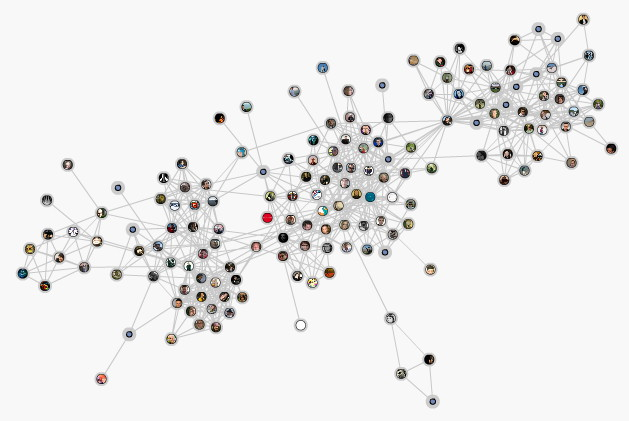
\includegraphics[scale=0.7]{img/facebook_social_graph.jpg}
}
\end{frame}

\begin{frame}
\frametitle{Grafo}
\frametitle{Disseminação de Doenças Infecciosas}
\resizebox{\textwidth}{!}{%
    \centering
    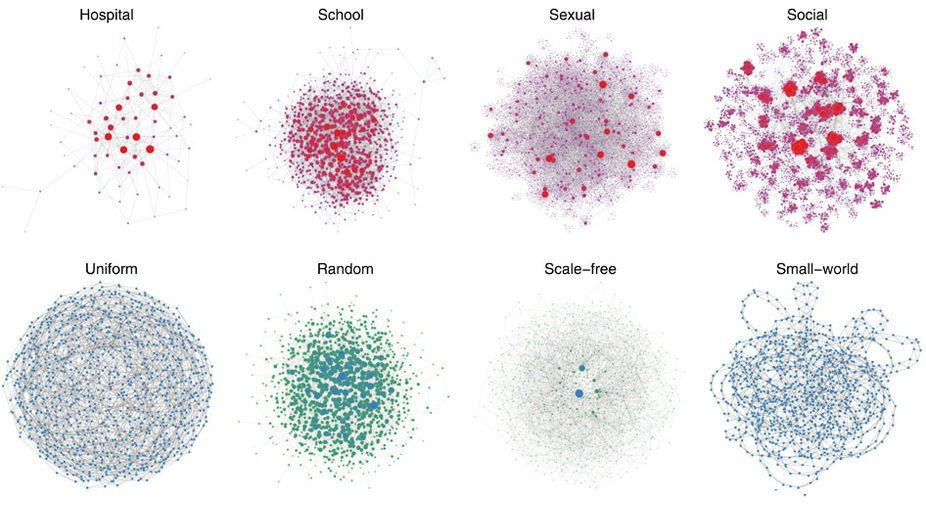
\includegraphics{img/ncomms7101-f2-a.jpg}
}
\end{frame}

\begin{frame}
\frametitle{Contaminação}
\framesubtitle{2-limitada}
\begin{columns}[T]
    \begin{column}{.75\textwidth}
       \resizebox{\textwidth}{!}{%
        \centering
        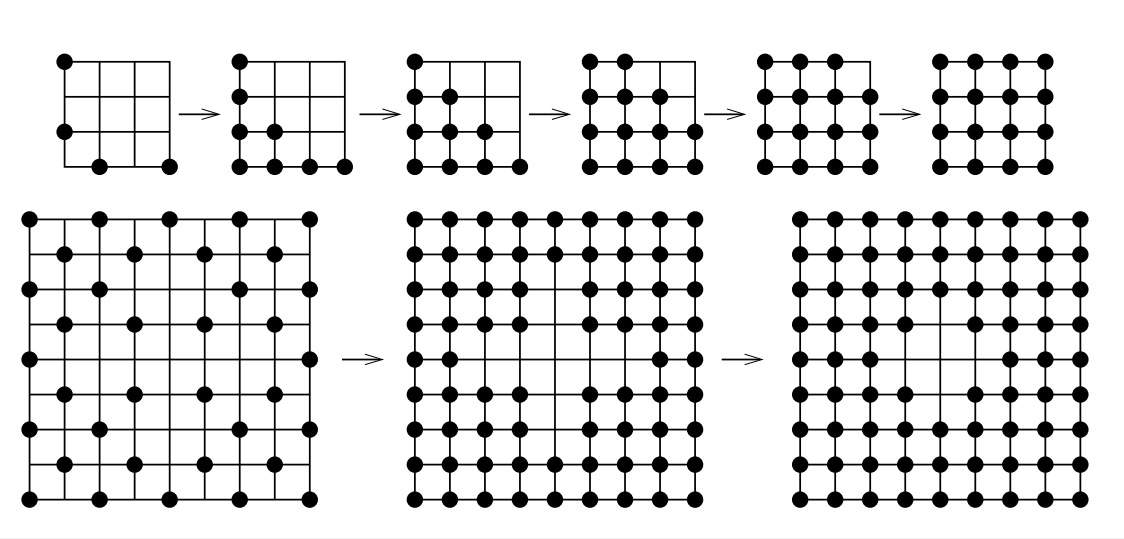
\includegraphics[scale=.5]{img/grid-contaminacao.png}
    }
    \end{column}
    \begin{column}{.25\textwidth}
        \begin{itemize}
            \item{Irreversível k-limitado: modelo de disseminação de doenças e opniões}
            \item{Irreversível 2-limitado}
        \end{itemize}
    \end{column}
  \end{columns}
\end{frame}

